\documentclass{article} % For LaTeX2e
\usepackage{nips15submit_e,times}
\usepackage{hyperref}
\usepackage{url}
\usepackage{amsthm, amsmath, bbm}
\usepackage{floatrow}
\newtheorem{theorem}{Theorem}
\usepackage{graphicx} % more modern
%\usepackage{epsfig} % less modern
\usepackage{subfigure} 
\usepackage{amsmath,amsfonts,amssymb}
\usepackage{tikz}
\usetikzlibrary{fit,positioning}
\usepackage[disable]{todonotes}

% For citations
\usepackage{natbib}

% For algorithms
\usepackage{algorithm}
\usepackage{algorithmic}

% As of 2011, we use the hyperref package to produce hyperlinks in the
% resulting PDF.  If this breaks your system, please commend out the
% following usepackage line and replace \usepackage{icml2015} with
% \usepackage[nohyperref]{icml2015} above.
\usepackage{hyperref}
\usepackage{tabularx}

% Packages hyperref and algorithmic misbehave sometimes.  We can fix
% this with the following command.
%\newcommand{\theHalgorithm}{\arabic{algorithm}}
\DeclareMathOperator{\Tr}{Tr}
%\newcommand{\R}{\mathbbm{R}}
\newcommand{\mba}{\mathbf{a}}
\newcommand{\mbb}{\mathbf{b}}
\newcommand{\mbx}{\mathbf{x}}
\newcommand{\mbxt}{\tilde{\mathbf{x}}}
\newcommand{\Sigmat}{\tilde{\Sigma}}
\newcommand{\mbz}{\mathbf{z}}
\newcommand{\mbw}{\mathbf{w}}
\newcommand{\mcN}{\mathcal{N}}
\newcommand{\mcP}{\mathcal{P}}
\newcommand{\mcX}{\mathcal{X}}
\newcommand{\eps}{\epsilon}
\newcommand{\trans}{\intercal}
\newcommand{\Ut}{\tilde{U}}
\DeclareMathOperator*{\argmax}{arg\,max}
\newcommand{\angstrom}{\textup{\AA}}
\newcommand{\red}[1]{\textcolor{red}{[TODO: #1]}}
\newcommand{\Nspec}{{N_{\text{spec}}}}
\newcommand{\Nphoto}{{N_{\text{photo}}}}

%%
%% figwidth, half figwidth
%%
\newlength{\figwidth}
\setlength{\figwidth}{6.75in}
\newlength{\halfwidth}
\setlength{\halfwidth}{3.37in}


%\documentstyle[nips14submit_09,times,art10]{article} % For LaTeX 2.09

\title{A Gaussian Process Model of Quasar \\ Spectral Energy Distributions}

\author{
Andrew Miller\thanks{\url{http://people.seas.harvard.edu/\~acm/}} \, ,  Albert Wu \\
School of Engineering and Applied Sciences\\
Harvard University\\
\texttt{acm@seas.harvard.edu, awu@college.harvard.edu}
\And
Jeffrey Regier, \, Jon McAuliffe \\
Department of Statistics \\
University of California, Berkeley \\
\texttt{\{jeff, jon\}@stat.berkeley.edu} \\
\And
Dustin Lang \\
McWilliams Center for Cosmology \\
Carnegie Mellon University \\
\texttt{dstn@cmu.edu} \\
\And
Prabhat, \, David Schlegel \\
Lawrence Berkeley National Laboratory \\
\texttt{\{prabhat, djschlegel\}@lbl.gov} \\
\And
Ryan Adams \thanks{\url{http://people.seas.harvard.edu/\~rpa/}}\\
School of Engineering and Applied Sciences\\
Harvard University\\
\texttt{rpa@seas.harvard.edu} \\
}

%\icmlauthor{Andrew Miller}{acm@seas.harvard.edu}
%\icmlauthor{Albert Wu}{awu@college.harvard.edu}
%\icmladdress{School of Engineering and Applied Sciences, Harvard University}
%\icmlauthor{Jeffrey Regier}{jeff@stat.berkeley.edu}
%\icmlauthor{Jon McAuliffe}{jon@stat.berkeley.edu}
%\icmladdress{Department of Statistics, University of California, Berkeley}
%\icmlauthor{Dustin Lang}{dstn@cmu.edu}
%\icmladdress{McWilliams Center for Cosmology, Carnegie Mellon University}
%\icmlauthor{Prabhat}{prabhat@lbl.gov}
%\icmlauthor{David Schlegel}{djschlegel@lbl.gov}
%\icmladdress{Lawrence Berkeley National Laboratory, 
%             1 Cyclotron Road, Berkeley, CA, 94720 USA}
%\icmlauthor{Ryan Adams}{rpa@seas.harvard.edu}
%\icmladdress{School of Engineering and Applied Sciences, Harvard University}

% The \author macro works with any number of authors. There are two commands
% used to separate the names and addresses of multiple authors: \And and \AND.
%
% Using \And between authors leaves it to \LaTeX{} to determine where to break
% the lines. Using \AND forces a linebreak at that point. So, if \LaTeX{}
% puts 3 of 4 authors names on the first line, and the last on the second
% line, try using \AND instead of \And before the third author name.

\newcommand{\fix}{\marginpar{FIX}}
\newcommand{\new}{\marginpar{NEW}}

%\nipsfinalcopy % Uncomment for camera-ready version

\begin{document}


\maketitle

\begin{abstract} 
We propose a method for combining two sources of astronomical data, spectroscopy and photometry, which carry information about sources of light (e.g., stars, galaxies, and quasars) at extremely different spectral resolutions. 
Our model treats the spectral energy distribution (SED) of the radiation from a source as a latent variable, hierarchically generating both photometric and spectroscopic observations.  
%Furthermore, we view the problem of SED inference as a density estimation problem, placing a flexible nonparametric prior over the SED of a light source that admits a physically interpretable decomposition and allows us to tractably perform Bayesian inference using Markov chain Monte Carlo (MCMC).  
We place a flexible, nonparametric prior over the SED of a light source that admits a physically interpretable decomposition, and allows us to tractably perform inference.  
We use our model to predict the distribution of the redshift of a quasar from five-band (low spectral resolution) photometric data, the so called ``photo-z'' problem. 
Our method shows that tools from machine learning and Bayesian statistics allow us to leverage multiple resolutions of information to make accurate predictions with well-characterized uncertainties. 
\end{abstract} 

\section{Introduction}
Enormous amounts of astronomical data are collected by a range of instruments at multiple spectral resolutions, providing information about billions of sources of light in the observable universe~\cite{alam2015eleventh, martin2005galex}.  
Among these data are measurements of the spectral energy distribution (SED) of a source.  
The SED describes the distribution of energy radiated by a source over the spectrum of wavelengths or photon energy levels.
The SED of a light source is of interest because it conveys information about its physical properties, including type, distance to the earth, and redshift, which will be an estimand of interest in this work. 
For intuition, the SED of a star at around 5,800 $K$ (e.g.,~the sun) radiates most of its energy in the 4,000 $\angstrom$ to 7,000 $\angstrom$ range, which corresponds roughly to the range of visible light.  
However, stars tend to have simple distributions (well-modeled by Planck's law), whereas other objects, such as galaxies and quasars, can have much more complicated SEDs.  

The SED can be thought of as a latent function for which we can only obtain noisy measurements.  Measurements of SEDs, however, are produced by instruments at widely varying spectral resolutions -- some instruments measure many wavelengths simultaneously (spectroscopy), while others average over large swaths of the energy spectrum and report a low dimensional summary (photometry). 
Spectroscopic data describe a source's SED in finer detail than broadband photometric data.  For example, the Baryonic Oscillation Spectroscopic Survey \cite{dawson2013baryon} measures SED samples at over four thousand wavelengths between 3,500 and 10,500 $\angstrom$.
In contrast, the Sloan Digital Sky Survey (SDSS)~\cite{alam2015eleventh} collects spectral information in only 5 broad spectral bins by using broadband filters (called $u,g,r,i,$ and $z$), but at a much higher \emph{spatial} resolution.  
Photometric preprocessing models can then aggregate pixel information into five band-specific fluxes and their uncertainties \cite{stoughton2002sloan}, reflecting the weighted average response over a large range of the wavelength spectrum. 
The two methods of spectral information collection are graphically compared in Figure~\ref{fig:filters}. 

%------ SDSS Filter Figure -----------------------------------------------
\begin{figure*}[t]
\vskip -.16in
\begin{center}
\subfigure{
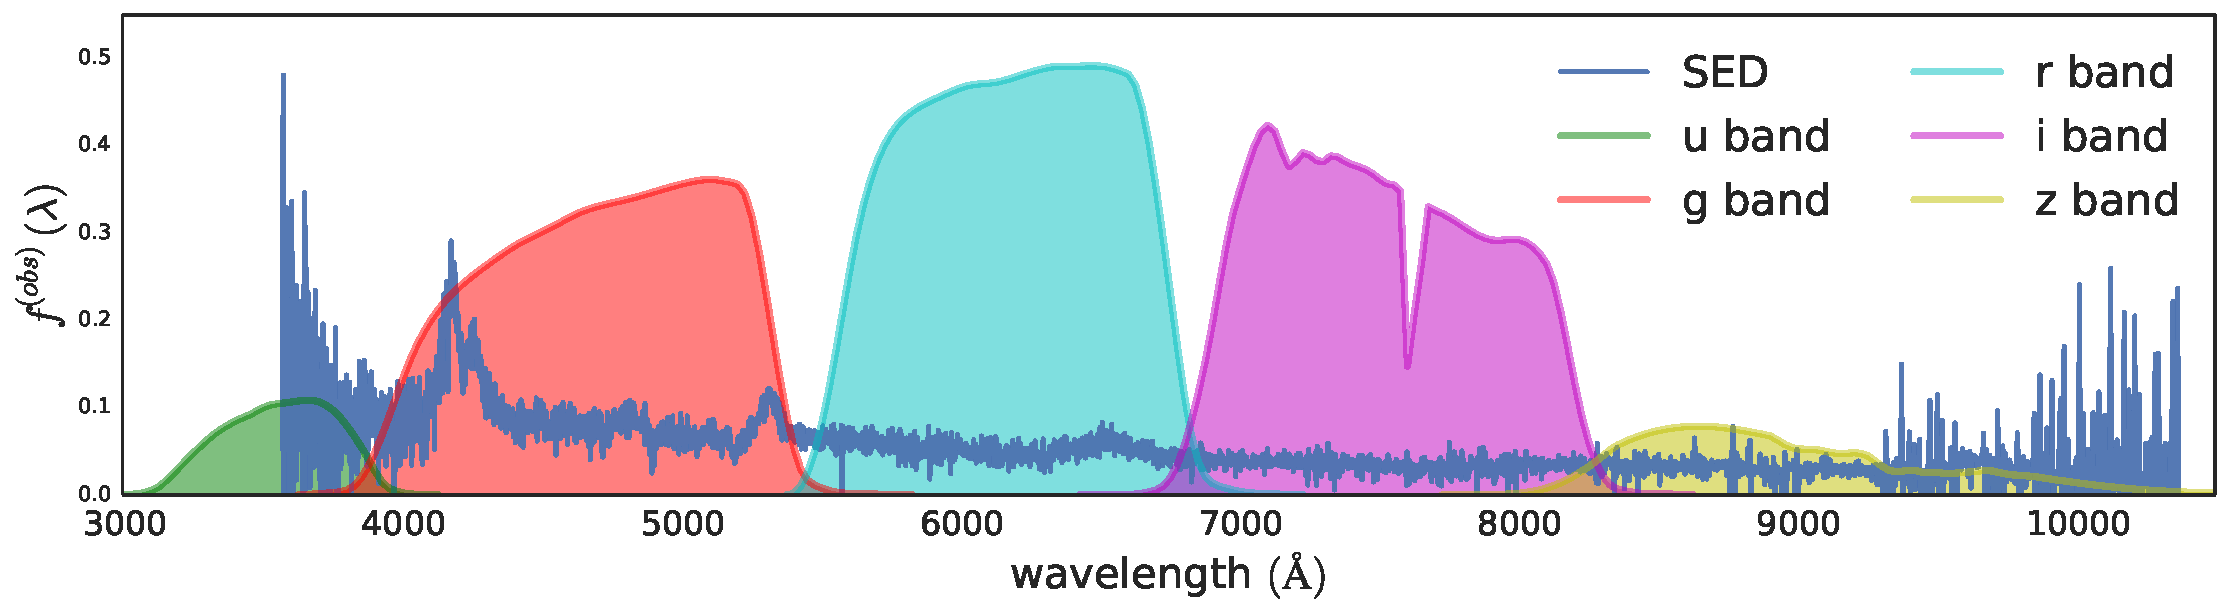
\includegraphics[width=.71\textwidth]{../figs/quasar_spectrum_sdss_filters}
}%
\subfigure{
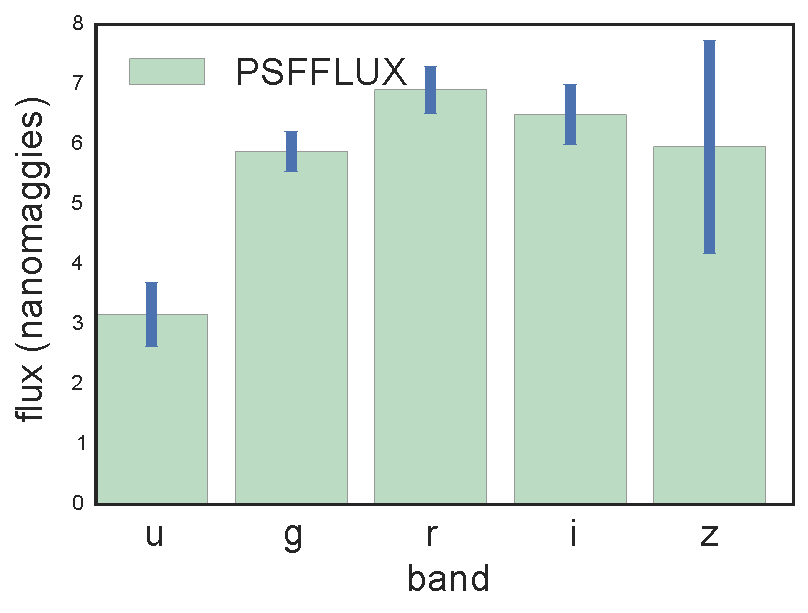
\includegraphics[width=.26\textwidth]{../figs/quasar_spectrum_bands}
}
\vskip -.16in
\caption{Left: example of a BOSS-measured quasar SED with SDSS band filters, $S_{b}(\lambda)$, $b \in \{u, g, r, i, z\}$, overlaid.  Right: the same quasar's photometrically measured band fluxes.  Spectroscopic measurements include noisy samples at thousands of wavelengths, whereas SDSS photometric fluxes reflect the (weighted) response over a large range of wavelengths.}
\label{fig:filters}
\end{center}
\end{figure*} 
\vskip -.1in
%--------------------------------------------------------------------------

Despite carrying less spectral information, broadband photometry is more widely available and exists for a larger number of sources than spectroscopic measurements. 
This work develops a method for extracting information from observations of light sources by jointly modeling spectroscopic and photometric data.  
One use of our model is to measure the redshift of quasars for which we only have photometric observations.  
Redshift is a phenomenon in which the observed SED of a source of light is stretched toward longer (redder) wavelengths.
This effect is due to a combination of radial velocity with respect to the observer and the expansion of the universe (termed \emph{cosmological redshift})~\cite{hogg1999distance, harrison1993redshift}.  
Quasars, or quasi-stellar radio sources, are extremely distant and energetic sources of electromagnetic radiation that can exhibit high redshift~\cite{silk1997quasars}.  
Accurate estimates and uncertainties of redshift measurements from photometry have the potential to guide the use of higher spectral resolution instruments to study sources of interest.  
Furthermore, accurate photometric models can aid the automation of identifying source types and estimating physical characteristics of faintly observed sources in large photometric surveys \cite{regier2015}.  

Our model jointly describes high-resolution spectroscopic data and low-resolution photometric observations of quasars in terms of their latent SEDs, apparent brightnesses, and redshifts. 
Representing a quasar's SED as a latent random measure, we describe a Bayesian inference procedure to compute the marginal probability distribution of a quasar's redshift given observed photometric fluxes and their uncertainties.  
The following section provides relevant application and statistical background.  
Section~\ref{sec:model} describes our probabilistic model of SEDs and broadband photometric measurements.
Section~\ref{sec:inference} outlines our MCMC-based inference method for efficiently computing statistics of the posterior distribution.
Section~\ref{sec:experiments} presents redshift and SED predictions from photometric measurements, among other model summaries, and a quantitative comparison between our method and two existing ``photo-z''.  
We conclude with a discussion and an outline of directions for future work.  

\section{Background}
\label{sec:background}
%The SED of a source describes the distribution of the energy it radiates as a function of wavelength.  
%For example, most stars are well-modeled as ideal black-body radiators, as their SED is well-described by a parametric form given by Planck's law. 
%The SEDs of most stars are approximately represented by Planck's law for black body radiators, and are well-described in detail by stellar atmosphere models \cite{gray2001physical}.  
The SEDs of most stars are approximately represented by Planck's law for black body radiators and stellar atmosphere models \cite{gray2001physical}. 
Quasars, on the other hand, have complicated SEDs characterized by some salient features, such as the Lyman-$\alpha$ forest, which is the absorption of light at many wavelengths from neutral hydrogen gas between the earth and the quasar~\cite{weinberg2003lymanalpha}.  
One of the most interesting properties of quasars (and galaxies) conveyed by the SED is redshift. 
Redshift affects our observation of SEDs by ``stretching'' the wavelengths, ${\lambda \in \Lambda}$, of the quasar's \emph{rest-frame} SED, skewing toward longer (redder) wavelengths.
Denoting the \emph{rest-frame} SED of a quasar~$n$ as a function,~${f_n^{(\text{rest})} : \Lambda \rightarrow \R_+}$, the effect of redshift with value $z_n$ (typically between 0 and 7) on the \emph{observation-frame} SED is described by the relationship 
\begin{align}
  f_n^{(\text{obs})}(\lambda) &= f_n^{(\text{rest})}\left(\frac{\lambda}{1 + z_n}\right) \, .
\end{align}
Some observed quasar spectra and their ``de-redshifted'' rest frame spectra are depicted in Figure~\ref{fig:frames}.

%------ example of obs vs rest frame data --------------------------------------
\begin{figure*}[t]
\vskip -.16in
\begin{center}
\centerline{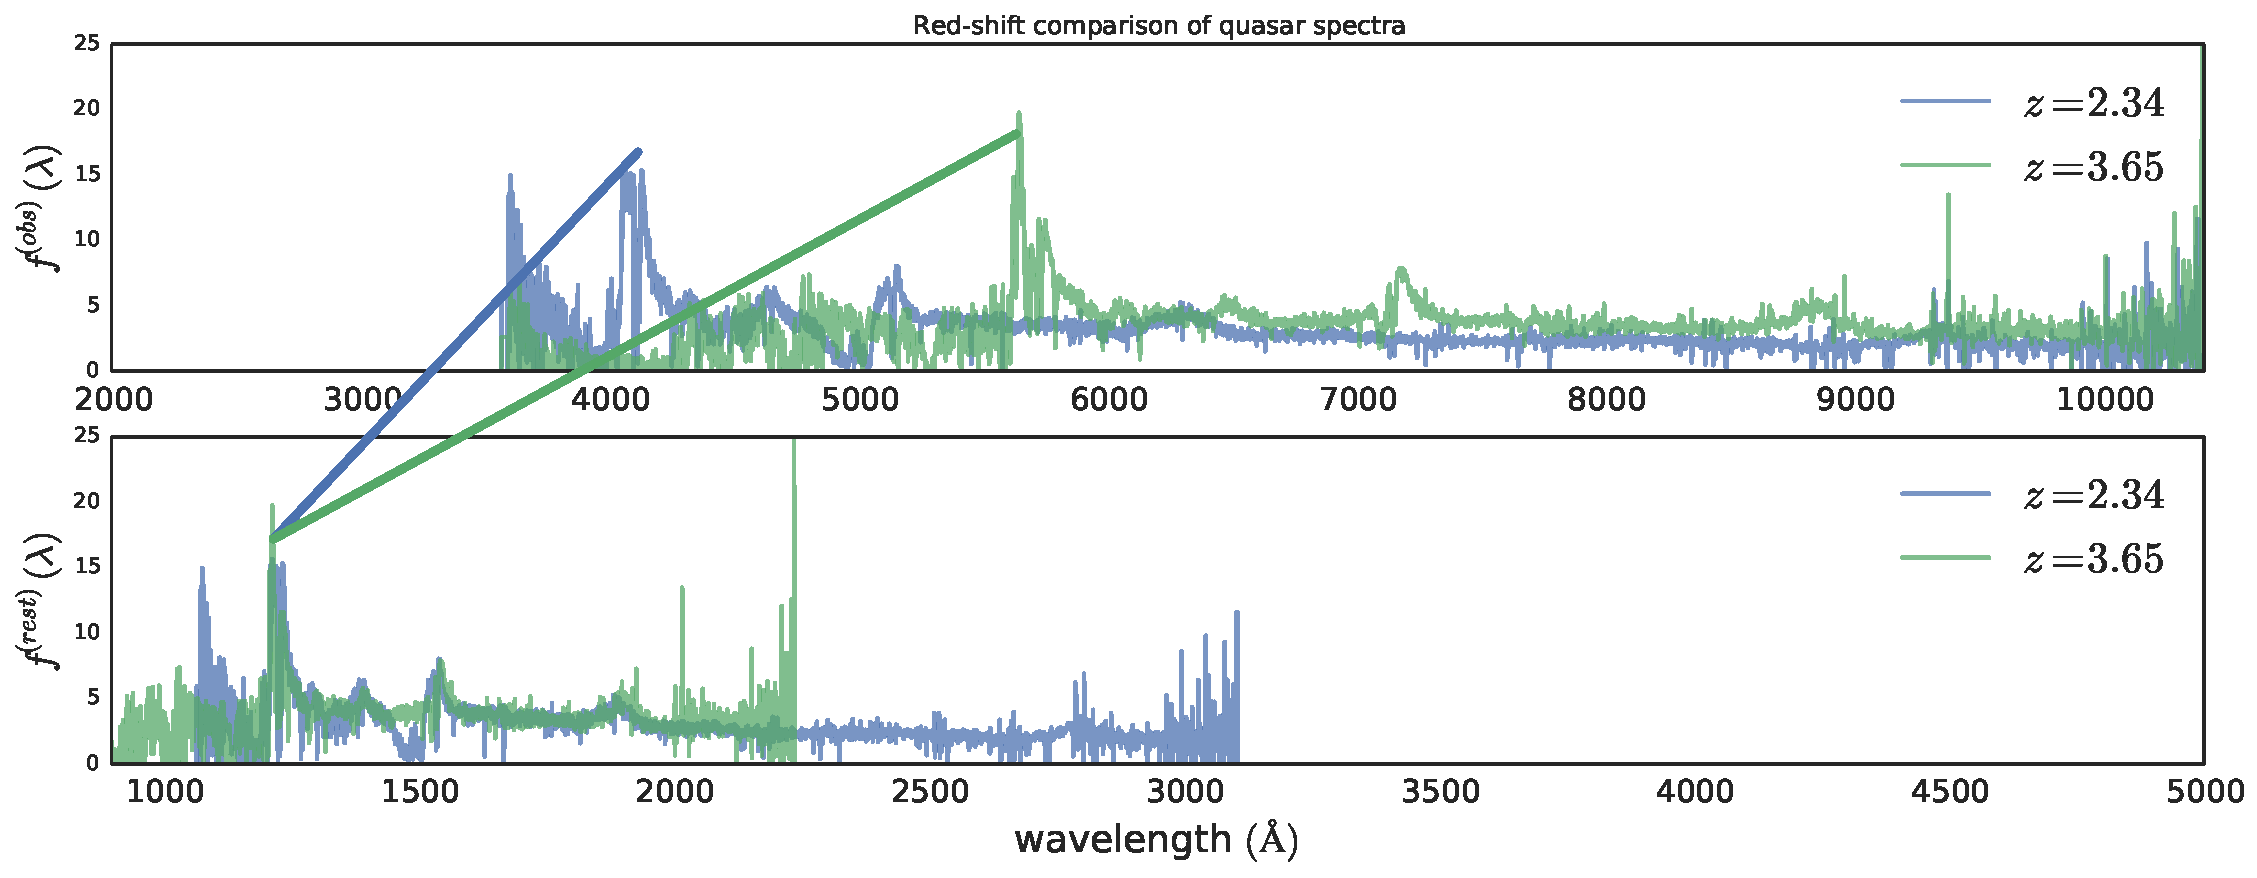
\includegraphics[width=.9\textwidth]{../figs/quasar_redshift_example}}
\vskip -.16in
\caption{%
Spectroscopic measurements of multiple quasars at different redshifts, $z$.
The upper graph depicts the sample spectrograph in the observation frame, intuitively thought of as ``stretched'' by a factor $(1+z)$.
The lower figure depicts the ``de-redshifted'' (rest-frame) version of the same quasar spectra, 
%This effectively squashes observations, and reconstructs each quasar spectrum as it would be seen in the quasar's rest frame.  
The two lines show the corresponding locations of the characteristic peak in each reference frame.  
Note that the $x$-axis has been changed to ease the visualization - the transformation is much more dramatic.  The appearance of translation is due to missing data; we don't observe SED samples outside the range 3,500-10,500 $\angstrom$.   
}
\vskip -.16in
\label{fig:frames}
\end{center}
\end{figure*} 


%\begin{figure}[t]
%\floatbox[{\capbeside\thisfloatsetup{capbesideposition={left,top},capbesidewidth=4.5cm}}]{figure}[.6\FBwidth]
%{ 
%\caption{%
%Spectroscopic measurements of multiple quasars at different redshifts, $z$.
%The top graphic depicts the sample spectrograph in the observation frame, intuitively thought of as ``stretched'' by a factor $(1+z)$.
%The lower figure depicts the ``de-redshifted'' version of the same quasar spectra.
%This effectively squashes observations, and reconstructs each quasar spectrum as it would be seen in the quasar's rest frame.  
%The two lines show the corresponding locations of the characteristic peak in each reference frame.  
%Note that the $x$-axis has been changed to ease the visualization - the transformation is much more dramatic.  The appearance of translation is due to missing data; we don't observe SED samples outside the range 3,500-10,500 $\angstrom$.   
%}
%  \label{fig:basis}
%}
%{
%  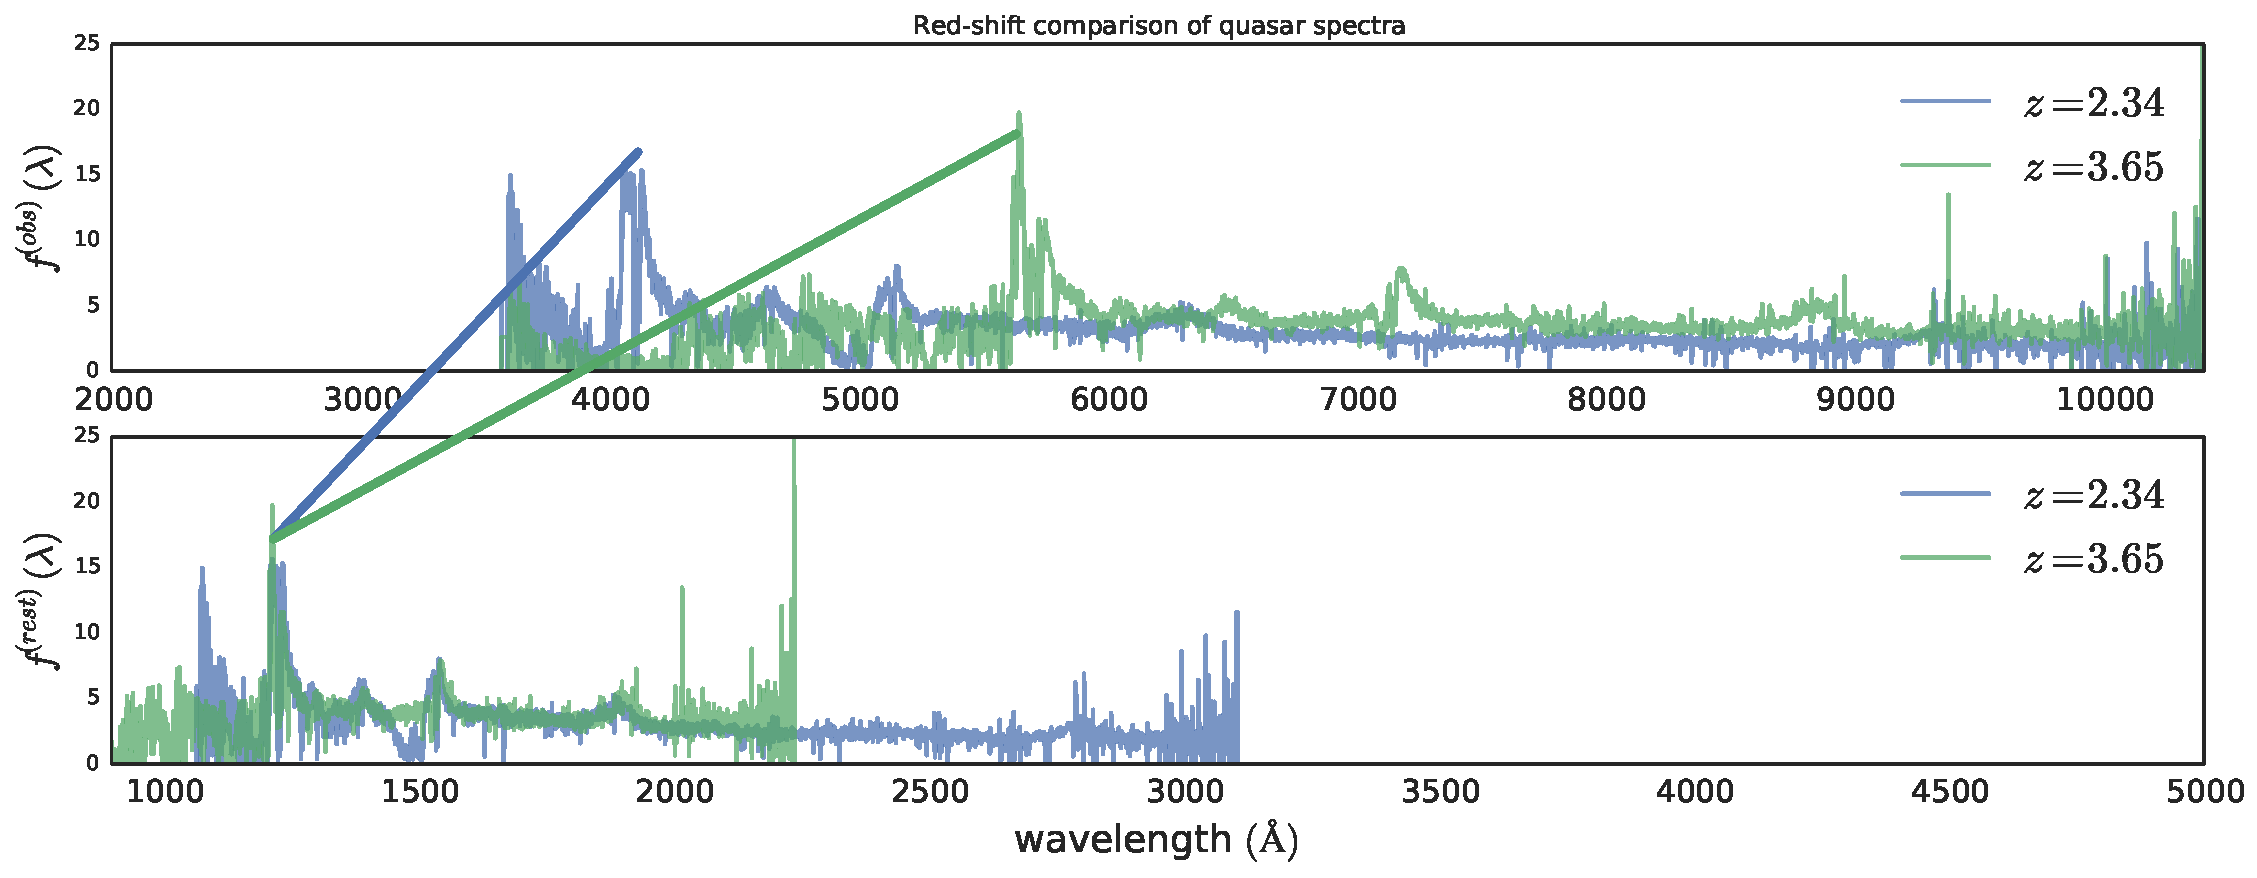
\includegraphics[width=.6\textwidth]{../figs/quasar_redshift_example}
%}
%\vskip -.16in
%\end{figure}
%--------------------------------------------------------------------------------


%----------------------------------------------------------------------------------
%----------------------------------------------------------------------------------
%----------------------------------------------------------------------------------
\section{Model}
\label{sec:model}
This section describes our probabilistic model of spectroscopic and photometric observations.  

\paragraph{Spectroscopic flux model}
The SED of a quasar is a non-negative function~${f : \Lambda \rightarrow \R^+}$, where~$\Lambda$ denotes the range of wavelengths and~$\R^+$ are non-negative real numbers representing flux density.
Our model specifies a quasar's \emph{rest-frame} SED as a latent random function. 
Quasar SEDs are highly structured, and we model this structure by imposing the assumption that each SED is a convex mixture of~$K$ latent, positive basis functions. 
The model assumes there are a small number of latent features or characteristics and that each quasar can be described by a short vector of mixing weights over these features.  
Following \cite{budavari2001photometric} we set ${K = 4}$, and note that this is also the number of PCA components that have been shown to carry over 90\% of the variation of quasar spectroscopy~\cite{suzuki2006quasar}.  
This value could also be fit using model-checking methods for latent factorization models, which we do not address for computational reasons.

We place a normalized log-Gaussian process prior (see~\ref{sec:gps}) on each of these basis functions.  
The generative procedure for quasar spectra begins with a shared basis
\begin{align}
  \beta_k(\cdot) &\stackrel{\text{iid}}{\sim} \mathcal{GP}(0, K_\theta),\; k=1, \dots, K,&
  B_k(\cdot) &= \frac{\exp(\beta_k(\cdot))}{\int_\Lambda \exp(\beta_k(\lambda))\, d\lambda}   \, ,
\end{align}
where $K_{\theta}$ is the kernel and $B_k$ is the exponentiated and normalized version of $\beta_k$. For each quasar~$n$,
\begin{align}
  \mathbf{w}_n &\sim p(\mathbf{w}) \, , \text{ s.t. } \sum_{w_k} w_k = 1, &
  m_n  &\sim p(m) \, , \text{ s.t. } m_n > 0, &
  z_n &\sim p(z),
\end{align}
where $\mathbf{w}_n$ mixes over the latent types, $m_n$ is the apparent brightness,~$z_n$ is the quasar's redshift, and distributions~$p(\mathbf{w})$,~$p(m)$, and~$p(z)$ are priors to be specified later.
As each positive SED basis function,~$B_k$, is normalized to integrate to one, and each quasar's weight vector~$\mathbf{w}_n$ also sums to one, the latent \emph{normalized} SED is then constructed as
\begin{align}
  f^{(\text{rest})}_n(\cdot) &= \sum_{k} w_{n,k} B_k(\cdot)
  \label{eqn:restsed}
\end{align}
and we define the unnormalized SED~${\tilde f^{(\text{rest})}_n(\cdot) \equiv m_n \cdot f^{(\text{rest})}_n(\cdot)}$. 
This parameterization admits the interpretation of~$f^{(\text{rest})}_n(\cdot)$ as a probability density scaled by $m_n$.  
This interpretation allows us to separate out the apparent brightness, which is a function of distance and overall luminosity, from the SED itself, which carries information pertinent to the estimand of interest, redshift. 

For each quasar with spectroscopic data, we observe noisy samples of the redshifted and scaled spectral energy distribution at a grid of $P$ wavelengths ${\lambda \in \{\lambda_1, \dots, \lambda_P \}}$.
For quasar $n$, our \emph{observation frame} samples are conditionally distributed as
\begin{align}
  x_{n, \lambda} | z_n, \mathbf{w}_n, \{ B_k \} 
    &\stackrel{\textrm{ind}}{\sim} \mathcal{N}\left( \frac{1}{1 + z_n} \tilde f_n^{(\text{rest})}\left( \frac{\lambda}{1 + z_n} \right), \sigma_{n,\lambda}^2 \right)
    \label{eq:spec} 
\end{align}
where $\sigma_{n, \lambda}^2$ is known measurement variance from the instruments used to make the observations, and the $1/(1+z_n)$ is a factor to preserve the overall volume of the rest-frame unnormalized SED. 
The BOSS spectra (and our rest-frame basis) are stored in units ${10^{-17} \cdot \text{erg} \cdot \text{cm}^{-2} \cdot \text{s}^{-1} \cdot \angstrom^{-1}}$.  

\paragraph{Gaussian process priors} 
\label{sec:gps}
Due to the complicated shape of quasar SEDs, we use a Gaussian process (GP) prior to flexibly encode our prior beliefs about their structure and shape.  A brief review of GPs is in the supplementary material.  
%
%A GP is a stochastic process,~${f: \mathcal{X} \rightarrow \R}$, such that any finite collection of random variables,~${f(x_1),\dots, f(x_N) \in \R}$, is distributed according to a multivariate normal distribution.  
%GPs are frequently used as priors over unknown functions, $f$, where the random variables $f(x_1), \dots, f(x_N)$ correspond to evaluations of the function at inputs ${x_1, \dots, x_N \in \mcX}$.  
%The covariance between any two outputs,~$f(x_i)$ and~$f(x_j)$, encodes prior beliefs about the function~$f$; carefully chosen covariance functions can encode beliefs about a wide range of properties, including smoothness and periodicity.  
%Throughout this paper we will use the the Mat\'{e}rn \cite{Matern1986spatial} covariance function
%\begin{align}
%  k_{\text{Matern}}(r)
%    &= \frac{2^{1-\nu}}{\Gamma(\nu)} 
%       \left( \frac{\sqrt{\nu} r}{\ell} \right) ^\nu
%       K_\nu\left( \frac{\sqrt{2\nu} r}{\ell}\right)
%\end{align}
%where ${r = |x_1 - x_2|}$, and $K_\nu$ is a modified Bessel function.  The parameter $\nu$ controls the smoothness and $\ell$ is the length scale of the function.  
%We choose the Mat\'{e}rn covariance function for its ability to trade off between smooth and flexible sample paths.  
%Because this covariance is strictly a function of the distance between two points in the space $\mcX$, it is said to be stationary. 
%See \cite{rasmussen2006gaussian} for a thorough treatment of Gaussian processes in machine learning. 

\paragraph{Photometric flux model }
Photometric data summarize the amount of energy observed over a large swath of the wavelength spectrum. 
Roughly, a photometric flux measures (proportionally) the number of photons hitting the instrument's lens over the duration of an exposure, filtered by a band-specific sensitivity curve. 
We express flux in nanomaggies~\cite{sdssnanomaggies}. 

Photometric fluxes and measurement error derived from broadband imagery have been computed directly from pixels \cite{stoughton2002sloan}.  
For each quasar $n$, SDSS photometric data are measured in five bands, ${b \in \{u,g,r,i,z\}}$, yielding a vector of five flux values and their variances,~$\mathbf{y}_n$ and~$\tau^2_{n, b}$.  
Each band, $b$, measures photon observations at each wavelength in proportion to a known filter sensitivity, $S_{b}(\lambda)$. 
The filter sensitivities for the SDSS $ugriz$ bands are depicted in Figure~\ref{fig:filters}, with an example observation frame quasar SED overlaid.  
The actual measured fluxes can be computed by integrating the full object's spectrum,~${m_n \cdot f_n^{(\text{obs})}(\lambda)}$ against the filters.
For a band~${b \in \{u, g, r, i, z \}}$
\begin{align}
  \mu_b(f_n^{(\text{rest})}, z_n) &= \int f^{(\text{obs})}_n(\lambda) \,S_b(\lambda)\, C(\lambda) \,d \lambda \,,
  & C(\lambda) = \frac{1}{\int S_b(\lambda) d\lambda} \frac{\lambda^2}{c} 10^{(48.6-2.5\cdot 17+22.5)/2.5} \,
\end{align}
where $C(\lambda)$ is a conversion factor to go from the units of~$f_n(\lambda)$ to nanomaggies
%\begin{equation*}
%C(\lambda) = \frac{1}{\int S_b(\lambda) d\lambda} \frac{\lambda^2}{c} 10^{(48.6-2.5\times 17+22.5)/2.5} \, .
%\end{equation*}
%\todo{Why doesn't the right hand side have a $\lambda$?}
The values in the expression above correspond to arbitrary zero-points and constants used in astronomical units: $48.6$ is a zero-point for an astronomical measurement called AB magnitude, $17$ is used to match fluxes which are in units of $10^{-17}$ ergs, $22.5$ and $2.5$ are constants used to convert from logarithmic to linear units of brightness, and $c$ is the speed of light in $\angstrom/s$.  

 We use $\mu_b$ to represent the full function from a rest spectrum and red shift to a band-specific flux.
 The results of this projection onto SDSS bands are modeled as independent Gaussian random variables with known variance
\begin{align}
  y_{n,b}\, |\, f_n^{(\text{rest})}, z_n 
    &\stackrel{\textrm{ind}}{\sim} 
      \mathcal{N}( \mu_b(f_n^{(\text{rest})}, z_n), \tau^2_{n,b} ) \, .
\end{align}
Conditioned on the basis, ${B = \{B_k\}}$, we can represent $f_n^{(\text{rest})}$ with a low-dimensional vector.
Note that~$f_n^{(\text{rest})}$ is a function of~${\mathbf{w}_n, z_n, m_n}$, and $B$~(see Equation~\ref{eqn:restsed}), so we can think of $\mu_b$ as a function of~${\mathbf{w}_n, z_n, m_n}$, and~$B$.
We overload notation, and re-write the conditional likelihood of photometric observations as
\begin{align}
    y_{n,b} \,|\, \mathbf{w}_n, z_n, m_n, B &\sim \mathcal{N}( \mu_b(\mathbf{w}_n, z_n, m_n, B), \tau^2_{n,b} ) \, .
   \label{eq:phot}
\end{align}
Intuitively, what gives us statistical traction in inferring the posterior distribution over $z_n$ is the structure learned in the latent basis $B$, i.e., the features that correspond to distinguishing bumps and dips in the SED.

%--- Graphical Model ------------------------------------------
%\begin{figure}
%\vskip -.16in
%
\tikzset{
  latentnode/.style={draw, minimum width=5mm, shape=circle, ultra thick, black},
  dagconn/.style={arrows=->, black, thick},
  plate/.style={draw, shape=rectangle, rounded corners=0.5ex, thick,
    minimum width=3.1cm, text width=3.1cm, align=right, inner sep=10pt, inner ysep=10pt,label={[xshift=-44pt,yshift=14pt]south east:#1}}
}

%\begin{figure}
\centering
\begin{tikzpicture}
\tikzstyle{main}=[circle, minimum size = 10mm, thick, draw =black!80, node distance = 12mm]
\tikzstyle{connect}=[-latex, thick]
\tikzstyle{box}=[rectangle, draw=black!100,label={[xshift=-14pt,yshift=14pt]south east:#1}]
  \node[main, fill = gray] (x) {$x_{n,\lambda}$};
  \node[main, fill=gray] (sigma) [below=of x] { $\sigma^2_{n,\lambda}$};
  \node[main, distance = 18mm] (w) [right=of x] {$\mathbf{w}_n$};
  \node[main, node distance = 5mm] (m) [below=of w] {$m_n$};
  \node[main, node distance = 5mm] (z) [below=of m] {$z_n$};
  \node[main, node distance = 18mm] (B) [above=of w] {$B_k$};
  \node[main] (ell) [left=of B] {$\ell, \nu$};
  \node[main, distance = 18mm, fill=gray] (y) [right=of w] {$y_{n,b}$};
  \node[main, fill=gray] (tau) [below=of y] {$\tau^2_{n,b}$};
  \path (B) edge [connect] (x)
           (B) edge [connect] (y)
           (w) edge [connect] (x)
           (w) edge [connect] (y)
           (m) edge [connect] (x)
           (m) edge [connect] (y)
           (z) edge [connect] (x)
           (z) edge [connect] (y)
           (sigma) edge [connect] (x)
           (tau) edge [connect] (y)
           (ell) edge [connect] (B) ;
    
  % draw plates
  \node[plate=, minimum width=26mm, inner sep=12pt, fit=(x) (sigma), label={[xshift=-34pt,yshift=14pt]south east:$\lambda \in \Lambda$}] (plate1) {};
  \node[plate=, minimum width=26mm, inner sep=12pt, fit=(y) (tau), label={[xshift=-73pt,yshift=16pt]south east:$b \in \{u,g,r,i,z\}$}] (plate1) {};
  \node[plate=, inner sep=15pt, fit=(B), label={[xshift=-15pt,yshift=14pt]south east:$K$}] (plate1) {};
  \node[plate, minimum width=31mm, minimum height=55mm, inner sep=4.4mm,draw=black!100, fit= (x) (sigma), label={[xshift=-29pt,yshift=14pt]south east:$N_{\text{spec}}$}] {};
  \node[plate, minimum width=31mm, minimum height=55mm, inner sep=4.4mm,draw=black!100, fit= (y) (tau), label={[xshift=-29pt,yshift=14pt]south east:$N_{\text{photo}}$}] {};
\end{tikzpicture}
%\end{figure}

%\vskip -.14in
%\caption{%
%Graphical model representation of the joint photometry and spectroscopy model. 
%The left shaded variables represent spectroscopically measured samples and their variances.
%The right shaded variables represent photometrically measured fluxes and their variances.
%Note that ${\Nspec + \Nphoto}$ replicates of $\mathbf{w}_n, m_n$ and $z_n$ are instantiated. }
%\label{fig:graphical}
%%\vskip -.16in
%\end{figure}
\begin{figure}[t]
\floatbox[{\capbeside\thisfloatsetup{capbesideposition={right,top},capbesidewidth=6cm}}]{figure}[\FBwidth]
{ 
  \caption{%
Graphical model representation of the joint photometry and spectroscopy model. 
The left shaded variables represent spectroscopically measured samples and their variances.
The right shaded variables represent photometrically measured fluxes and their variances.  The upper box represents the latent basis, with GP prior parameters $\ell$ and $\nu$.  
Note that ${\Nspec + \Nphoto}$ replicates of $\mathbf{w}_n, m_n$ and $z_n$ are instantiated. }
  \label{fig:graphical}
}
{\resizebox{4.5cm}{!}{%
  
\tikzset{
  latentnode/.style={draw, minimum width=5mm, shape=circle, ultra thick, black},
  dagconn/.style={arrows=->, black, thick},
  plate/.style={draw, shape=rectangle, rounded corners=0.5ex, thick,
    minimum width=3.1cm, text width=3.1cm, align=right, inner sep=10pt, inner ysep=10pt,label={[xshift=-44pt,yshift=14pt]south east:#1}}
}

%\begin{figure}
\centering
\begin{tikzpicture}
\tikzstyle{main}=[circle, minimum size = 10mm, thick, draw =black!80, node distance = 12mm]
\tikzstyle{connect}=[-latex, thick]
\tikzstyle{box}=[rectangle, draw=black!100,label={[xshift=-14pt,yshift=14pt]south east:#1}]
  \node[main, fill = gray] (x) {$x_{n,\lambda}$};
  \node[main, fill=gray] (sigma) [below=of x] { $\sigma^2_{n,\lambda}$};
  \node[main, distance = 18mm] (w) [right=of x] {$\mathbf{w}_n$};
  \node[main, node distance = 5mm] (m) [below=of w] {$m_n$};
  \node[main, node distance = 5mm] (z) [below=of m] {$z_n$};
  \node[main, node distance = 18mm] (B) [above=of w] {$B_k$};
  \node[main] (ell) [left=of B] {$\ell, \nu$};
  \node[main, distance = 18mm, fill=gray] (y) [right=of w] {$y_{n,b}$};
  \node[main, fill=gray] (tau) [below=of y] {$\tau^2_{n,b}$};
  \path (B) edge [connect] (x)
           (B) edge [connect] (y)
           (w) edge [connect] (x)
           (w) edge [connect] (y)
           (m) edge [connect] (x)
           (m) edge [connect] (y)
           (z) edge [connect] (x)
           (z) edge [connect] (y)
           (sigma) edge [connect] (x)
           (tau) edge [connect] (y)
           (ell) edge [connect] (B) ;
    
  % draw plates
  \node[plate=, minimum width=26mm, inner sep=12pt, fit=(x) (sigma), label={[xshift=-34pt,yshift=14pt]south east:$\lambda \in \Lambda$}] (plate1) {};
  \node[plate=, minimum width=26mm, inner sep=12pt, fit=(y) (tau), label={[xshift=-73pt,yshift=16pt]south east:$b \in \{u,g,r,i,z\}$}] (plate1) {};
  \node[plate=, inner sep=15pt, fit=(B), label={[xshift=-15pt,yshift=14pt]south east:$K$}] (plate1) {};
  \node[plate, minimum width=31mm, minimum height=55mm, inner sep=4.4mm,draw=black!100, fit= (x) (sigma), label={[xshift=-29pt,yshift=14pt]south east:$N_{\text{spec}}$}] {};
  \node[plate, minimum width=31mm, minimum height=55mm, inner sep=4.4mm,draw=black!100, fit= (y) (tau), label={[xshift=-29pt,yshift=14pt]south east:$N_{\text{photo}}$}] {};
\end{tikzpicture}
%\end{figure}

  } 
}
\vskip -.16in
\end{figure}
%------------------------------------------

%\subsection{Joint model}
%Given a sample of $\Nspec$ noisy full spectra and their sample locations, ${\mathbf{X} \equiv \{\mathbf{x}_n, \lambda^{(\text{obs})}_n \}}$, and a set of~$\Nphoto$ photometric fluxes,~${\mathbf{Y} \equiv \{\mathbf{y}_n\}}$, our full likelihood in terms of~$\{ \mathbf{w}_n, z_n, m_n \}, \{ B_1, \dots, B_K \}$ is 
%\begin{align*}
%  L( \{ \mathbf{w}_n, ~&z_n, m_n \}, \{ B_k \} )
%    = & \prod_{n=1}^\Nspec p( \mathbf{x}_n | \mathbf{w}_n, z_n, m_n, \{ B_k \})
%        \prod_{n=\Nspec+1}^{\Nspec + \Nphoto} p( \mathbf{y}_n | \mathbf{w}_n, z_n, m_n, \{ B_k \})\,,
%\end{align*}
%where the probability distribution of the first factor in the product is given by Equation~\ref{eq:spec}, and the distribution for the second factor in the product is given by Equation~\ref{eq:phot}.  
%Whether measured spectroscopically or photometrically, all of the quasars' SEDs share the same basis, hierarchically tying them together.
%This basis provides a highly compact representation of a quasar SED, and is what drives photometric redshift predictions.  
%The joint distribution is depicted as a graphical model in Figure~\ref{fig:graphical}.

\paragraph{Note on priors}
For photometric weight and redshift inference, we use a flat prior on $z_n$, and empirically derived priors for $m_n$ and $w_n$, from the sample of spectroscopically measured sources.  
We fit a mixture of Gaussians to the logit space variables, $\omega$, defined 
\begin{align}
  \omega_k &\sim \mathcal{N}(0, 1), \, k = 1, \dots, K-1 &
  w_k &= \frac{\exp(\omega_k)}{1 + \sum_{k'} \exp(\omega_{k'})} \, .
\end{align}
We fit this prior on the $\omega$ weights derived from the full spectroscopically measured dataset.  We determine the number of components by comparing likelihoods on a held-out validation set.  

% and a log-Gaussian process prior over each basis  o
%We express the joint prior distribution over weights $\mathbf{w}_n$, $\mathbf{w}_m$, and %basis $\{B_k\}$ as:
%\begin{align}
%  p( \{ \mathbf{w}_m, z_m \}, &\{ B_k \}, \{ \mathbf{w}_n, z_n \} )  \\
%    = & p(\{ B_k \}) p( \{ \mathbf{w}_m, z_m \} )  \\
%      & p( \{ \mathbf{w}_n, z_n \} | \{ \mathbf{w}_m, z_m \} ) 
%\end{align}
%where we condition the photometric weights on the spectroscopically fit weights.  

%---- TABLE, coverage --------------------------------------
%\begin{table*}[t]
%\caption{%
%Top: mean absolute and mean absolute percentage error of photometric redshift predictions with respect to spectroscopic ``ground truth''.
%Bottom: number of predicted values covered by posterior sample quantiles of varying size. }
%\label{tab:error}
%\vskip 0in
%\begin{center}
%\begin{small}
%\begin{sc}
%\begin{center}
%\begin{tabular*}{0.95\textwidth}{cccccccc} 
\hline\abovespace\belowspace 
$z_{spec}$ & $ > 0.0 (1992)$ & $ > 1.0 (1832)$ & $ > 2.0 (1734)$ & $ > 3.0 (1127)$ & $ > 4.0 (995)$ & $ > 4.5 (321)$ & $ > 5.0 (43)$\\ 
\hline 
\abovespace 
mean MAE & 0.39 & 0.35 & 0.35 & 0.27 & 0.25 & 0.27 & 0.35 \\ 
mode MAE & 0.50 & 0.47 & 0.46 & 0.36 & 0.34 & 0.27 & 0.39 \\ 
mean MAPE & 0.21 & 0.12 & 0.11 & 0.06 & 0.06 & 0.06 & 0.07 \\ 
mode MAPE & 0.24 & 0.17 & 0.15 & 0.09 & 0.08 & 0.06 & 0.08 \\ 
\hline 
\% in [.5, 99.5] & 86.1 & 86.5 & 86.4 & 80.5 & 79.2 & 75.7 & 69.8 \\ 
\% in [5, 95] & 74.6 & 74.9 & 74.7 & 67.1 & 65.2 & 56.7 & 46.5\\ 
 \hline\end{tabular*}
%\end{center}
%\end{sc}
%\end{small}
%\end{center}
%\vskip -0.1in
%\end{table*}
%------------------------------------------------------------------------------


%----------------------------------------------------------------------------------
%----------------------------------------------------------------------------------
%----------------------------------------------------------------------------------
\section{Inference}
\label{sec:inference} 
%For example, to compute expectations with respect to the marginal posterior distribution over quasar redshift, we will want to produce posterior samples of $z_n$, $\mathbf{w}_n$, and $B$, yielding Monte Carlo approximations
%\begin{align}
%  \mathbb{E}[ g(z_n) | \mathbf{y}_n, \mathbf{X} ] 
%    &\approx \frac{1}{N} \sum_{i} g(z_n^{(i)}) \\
%    z_n^{(i)}, \mathbf{w}_n | \mathbf{y}_n, B &\sim p(z_n, \mathbf{w}_n^{(i)} | \mathbf{y}_n, B) 
    %B^{(i)} &\sim p(B | \mathbf{X}, \mathbf{Y}) \, 
%\end{align}
%where $g$ represents an arbitrary function of redshift, and $N$ is the total number of Monte Carlo samples.  
\paragraph{Basis estimation}
For computational tractability, we first compute a maximum a posteriori (MAP) estimate of the basis,~$B_{\text{map}}$ to condition on.  
Using the spectroscopic data, $\{x_{n, \lambda}, \sigma_{n, \lambda}^2, z_n\}$, we compute a discretized MAP estimate of $\{B_k\}$ by directly optimizing the unnormalized (log) posterior implied by the likelihood in Equation~\ref{eq:spec}, the GP prior over $B$, and diffuse priors over $\mathbf{w}_n$ and $m_n$,
\begin{align}
	p\left(\{\mathbf{w}_n, m_n\}, \{ B_k \} | \{x_{n, \lambda}, \sigma_{n, \lambda}^2, z_n\} \right) 
	&\propto \prod_{n=1}^N p(x_{n, \lambda} | z_n, \mathbf{w}_n, m_n, \{B_k\}) p(\{B_k\}) p(\mathbf{w}_n) p(m_n) \, .
\end{align}
We use gradient descent with momentum and LBFGS \cite{nocedal1980updating} directly on the parameters $\beta_k, \omega_{n,k}$, and $\log(m_n)$ for the $N_{spec}$ spectroscopically measured quasars.  
Following \cite{walcher2011fitting}, we first resample the observed spectra into a common rest-frame grid, ${\lambda_0 = (\lambda_{0,1}, \dots, \lambda_{0,V})}$, easing computation of the likelihood.  
We note that although our model places a full distribution over~$B_k$, efficiently integrating out those parameters is left for future work.

%The following section outlines our MCMC procedure to compute posterior samples of $\mathbf{w}_n, z_n$, and $m_n$ given the sample of spectra, $\mathbf{X}$, photometric fluxes $\mathbf{y}_{ugriz}$, and $B_{\text{map}}$.

%\subsection{Sampling $B$}
%To accelerate computation, we use only information present in $\mathbf{X}$ to draw samples of $B_1, \dots, B_K$.  That is, we approximate the full conditional distribution 
%\begin{align}
%  p(B_1,\dots, B_k | \mathbf{X}, \mathbf{Y}) 
%    &\approx p(B_1, \dots, B_k | \mathbf{X})
%\end{align}
%We expect this to have little effect on the distribution, as the amount of information about $B$ present in $\mathbf{X}$, the high-resolution full-spectrum data, is expected to dwarf that of $\mathbf{Y}$, the
%low-resolution bandwise fluxes.  The posterior distribution from which we sample, $p(B | \mathbf{X})$, can be written 
%\begin{align}
%  p(B | \mathbf{X}) 
%    &\propto p(\mathbf{X} | \{ \mathbf{w}_m\}_{m=1}^M, B) p(\beta) p(\mathbf{w}) \, .
%\end{align}
%We draw posterior samples using Hamiltonian Monte Carlo \cite{neal2011mcmc}, an auxiliary variable method that uses gradient information to efficiently mix.  Empirically, naive Metropolis-Hastings mixes too slowly for practical purposes. 

\paragraph{Sampling $\mathbf{w}_n, m_n$, and $z_n$}
The Bayesian ``photo-z'' task requires that we compute posterior marginal distributions of $z$, integrating out $\mathbf{w}$, and $m$.  
To compute these distributions, we construct a Markov chain over the state space including $z$, $\mathbf{w}$, and $\mathbf{m}$ that leaves the target posterior distribution invariant.
%and condition similar to Monte Carlo EM~\cite{wei1990monte}
We treat the inference problem for each photometrically measured quasar, $\mathbf{y}_n$, independently.
Conditioned on a basis~${B_k, k=1,\dots, K}$, our goal is to draw posterior samples of $\mathbf{w}_n$, $m_n$ and $z_n$ for each $n$.  
The unnormalized posterior can be expressed
\begin{align}
  p(\mathbf{w}_n, m_n, z_n | \mathbf{y}_n, B)
  &\propto p(\mathbf{y}_n | \mathbf{w}_n, m_n, z_n, B) p(\mathbf{w}_n, m_n, z_n) \end{align}
where the left likelihood term is defined in Equation~\ref{eq:phot}. 
Note that due to analytic intractability, we numerically integrate expressions involving $\int_\Lambda f_n^{(obs)}(\lambda) d\lambda$.
Because the observation $\mathbf{y}_n$ can often be well explained by various redshifts and weight settings, the resulting marginal posterior, $p(z_n | \mathbf{X}, \mathbf{y}_n, B)$, is often multi-modal, with regions of near zero probability between modes.
Intuitively, this is due to the information loss in the SED-to-photometric flux integration step.

This multi-modal property is problematic for many standard MCMC techniques. 
Naive Metropolis-Hastings would have to jump between modes or travel through a region of near-zero probability, resulting in slow mixing.  
To combat this effect, we use parallel tempering \cite{brooks2011handbook}, a method that is well-suited to constructing Markov chains on multi-modal distributions.
Parallel tempering instantiates~$C$ independent chains, each sampling from the target distribution raised to an inverse temperature.
Given a target distribution, $\pi(x)$, the constructed chains sample 
${\pi_c(x) \propto \pi(x)^{1/T_c}}$,
where~$T_c$ controls how ``hot'' (i.e.,~how close to uniform) each chain is. 
At each iteration, swaps between chains are proposed and accepted with a standard Metropolis-Hastings acceptance probability 
\begin{align}
  \Pr(\text{accept swap } c, c') = \frac{ \pi_c(x_{c'}) \pi_{c'}(x_c) }{ \pi_c(x_c) \pi_{c'}(x_{c'}) } \, .
\end{align}
Within each chain, we use component-wise slice sampling \cite{neal2003slice} to generate samples that leave each chain's distribution invariant.  Slice-sampling is a (relatively) tuning-free MCMC method, a convenient property when sampling from thousands of independent posteriors.  


%---------------------------------------------------------------------------------
%---------------------------------------------------------------------------------
%---------------------------------------------------------------------------------
%\section{Related work}
%\label{sec:related}
%Many machine learning and statistical methods have been applied to the ``photo-$z$'' problem. The review by \cite{walcher2011fitting} divides ``photo-$z$'' methods into two categories, empirical and template-fitting.  Empirical methods are often discriminative, regression-based approaches, whereas template-fitting methods are often SED model-based approaches.  
%
%A recently proposed empirical method uses a multi-layer perceptron with a combination of photometric datasets, including SDSS, 
%%SDSS, UKIDSS, and WISE photometric fluxes datasets, 
%to compute a regression function for redshift \cite{brescia2013photometric}. 
%This method, while efficient and accurate in mean error, does not characterize the uncertainty of the estimated redshift, nor does it admit any physically interpretable estimate of the SED and quasar type.  
%Template-based approaches use information derived from spectroscopy to assist redshift predictions.  
%\cite{budavari2001photometric} and \cite{richards2001photometric} present a clustering algorithm for reconstructing quasar SEDs from photometric observations and templates derived from noisy spectroscopic measurements.  
%Their method clusters quasars into individual template categories using a $K$-means-like update, relying on weighted template averages of noisy SED measurements and unique cluster assignments that do not express uncertainty over quasar ``types''. 
%Instead of a pure clustering method, we use a non-negative factor analysis-type model to represent the latent structure of quasar SEDs and a continuous, low-dimensional range of quasar types.  
%Furthermore, our method presents a fully probabilistic model of SEDs and a Bayesian inference procedure that integrates out uncertainty over latent variables, including quasar type and apparent brightness, to measure redshift.    
%
%Other models blur the line between regression-based and generative models. \cite{bovy2012photometric} develops the $XDQSOz$ method to use a large dataset of astronomical objects to simultaneously infer redshift and classify quasars.  
%They model the joint distribution over object type, fluxes, and redshift.  However, their method does not model SEDs themselves, nor the SED-to-flux generative process. 
%They do this by inferring a joint distribution over object type, fluxes, and redshift. In particular, they factor this joint distribution
%into one part that describes the distribution over star brightness, which involves binning based on a single-channel flux, and
%one part that describes the distribution of relative fluxes (as compared to this channel) and the redshift. The latter distribution
%is represented by a mixture of up to 60 Gaussians. 
%However, we see that, due to the
%binning, this approach is not fully probabilistic or Bayesian.

%\citet{benitez2000bayesian} presents a thorough summary of Bayesian methods for photometric redshift estimation from spectral templates.  
%\citet{budavari2009unified} unifies template-based and regression-based
%approaches into a single probabilistic framework, distinguishing methods based on the assumptions they impose on probability distributions over photometric fluxes. 

%\red{Others to mention: }
%\cite{suzuki2006quasar} does unsupervised learning on the UV spectra of quasars using principal components analysis (PCA). Through this analysis, the authors found that 96\% of the total variance was accounted for by the first 3 spectral components. As a result, they created a classification scheme based on the first two component's coefficients that separates quasars into five different classes. This classification scheme allows researchers to understand quasars better from a qualitative perspective.
%\red{This doesn't seem that relevant. What do you think, Andy?}



%----------------------------------------------------------------------------------
%----------------------------------------------------------------------------------
%----------------------------------------------------------------------------------
\section{Experiments and Results}
\label{sec:experiments}
We fit our model to three training sets composed of spectroscopically measured quasars from the DR10QSO dataset \cite{paris2014sloan} with confirmed redshifts in the range ${z \in (.01,  5.85)}$.  
Our experiments split the data in three ways: (i) randomly, (ii) by $r$-band fluxes, (iii) by redshift values.  In split (ii), we train on the brightest 90\% of quasars, and test on a subset of the remaining.  Split (iii) takes the lowest 85\% of quasars as training data, and a subset of the brightest 15\% as test cases.  Splits (ii) and (iii) are intended to test the method's robustness to different training and testing distributions, mimicking the discovery of fainter and farther sources.  
For each split, we find a MAP estimate of the basis, $B_1, \dots, B_K$, and weights, $\mathbf{w}_n$ to use as a prior for photometric inference.  For computational purposes, we limit our training sample to a random subsample of 2,000 quasars.   
The following sections outline the resulting model fit and inferred SEDs and redshifts. 

%----- -------------------------------------------------
\begin{figure}[t]
\vskip -.1in
\floatbox[{\capbeside\thisfloatsetup{capbesideposition={right,top},capbesidewidth=5.5cm}}]{figure}[\FBwidth]
{ 
  \caption{%
Top: MAP estimate of the latent bases ${B = \{B_k\}_{k=1}^K}$.
Note the different ranges of the $x$-axis (wavelength).
Each basis function distributes its mass across different regions of the spectrum to explain different salient features of quasar spectra in the rest-frame.
Bottom: model reconstruction of a training-sample SED. }
  \label{fig:basis}
}
{
  \hskip -.2in 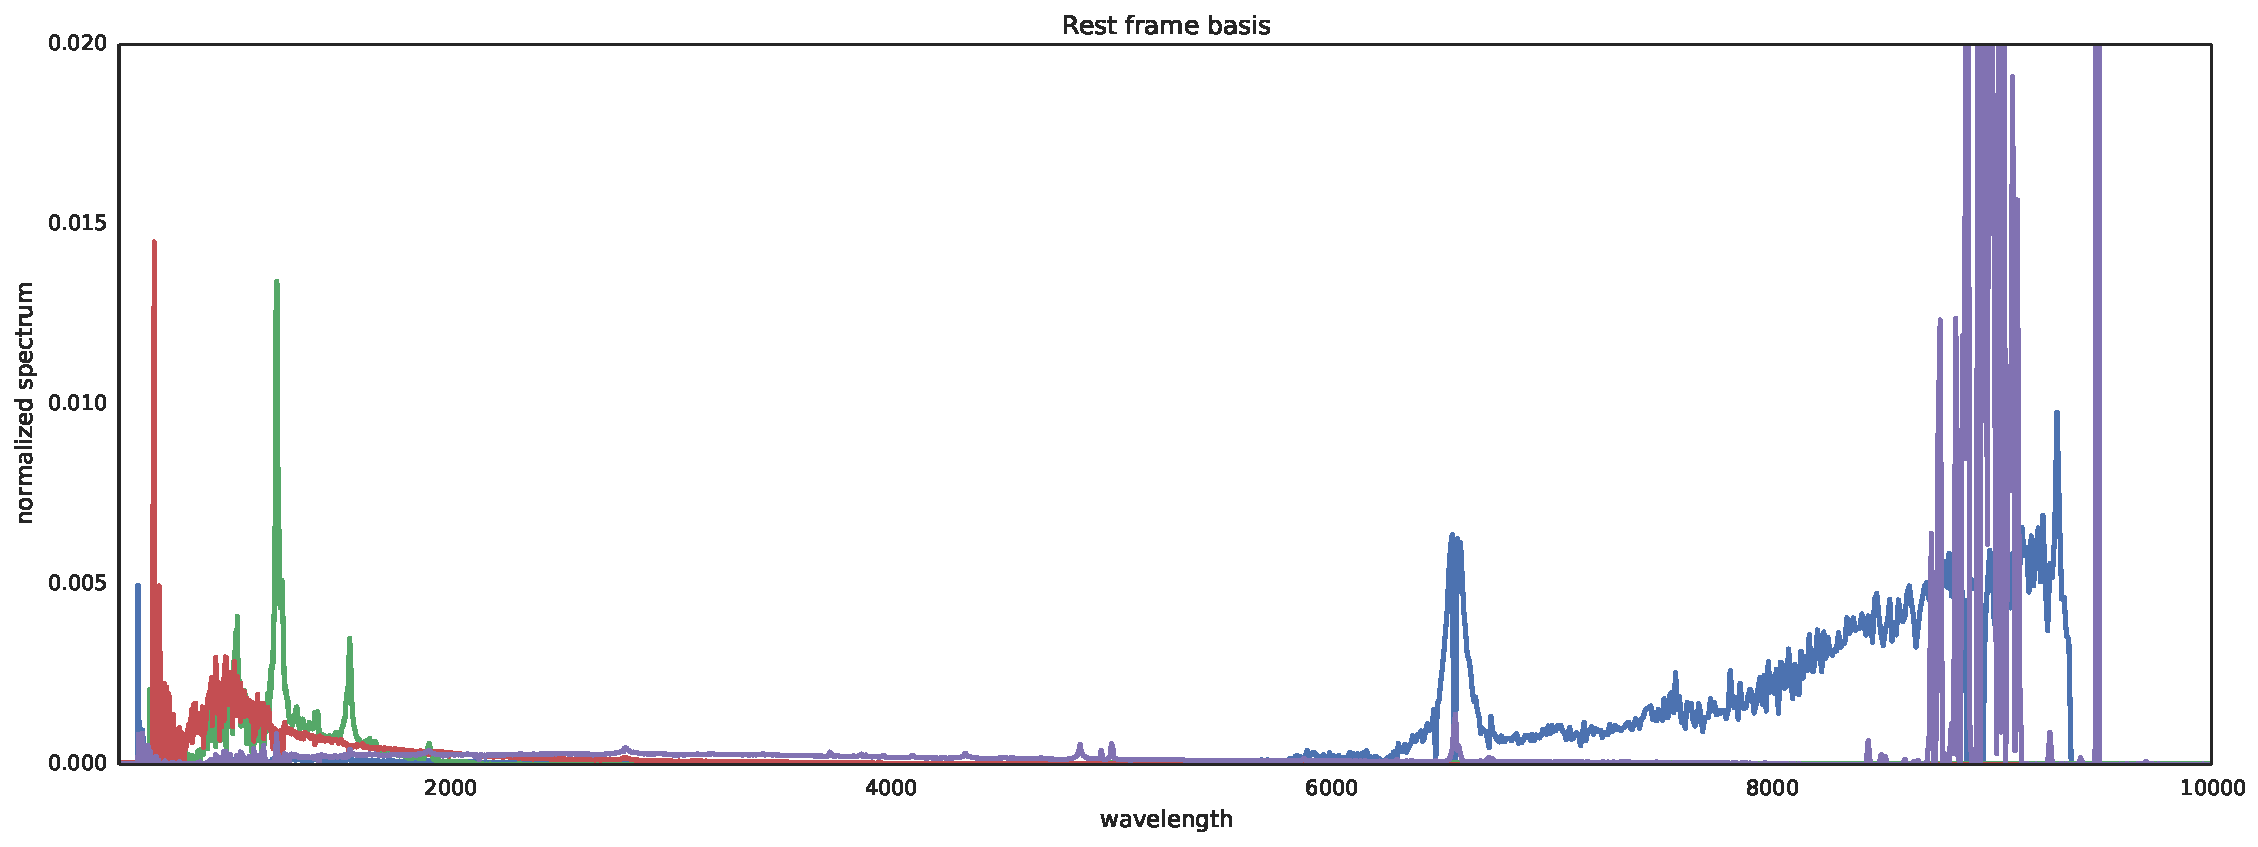
\includegraphics[width=.55\textwidth]{../figs/rank_4_basis}
}
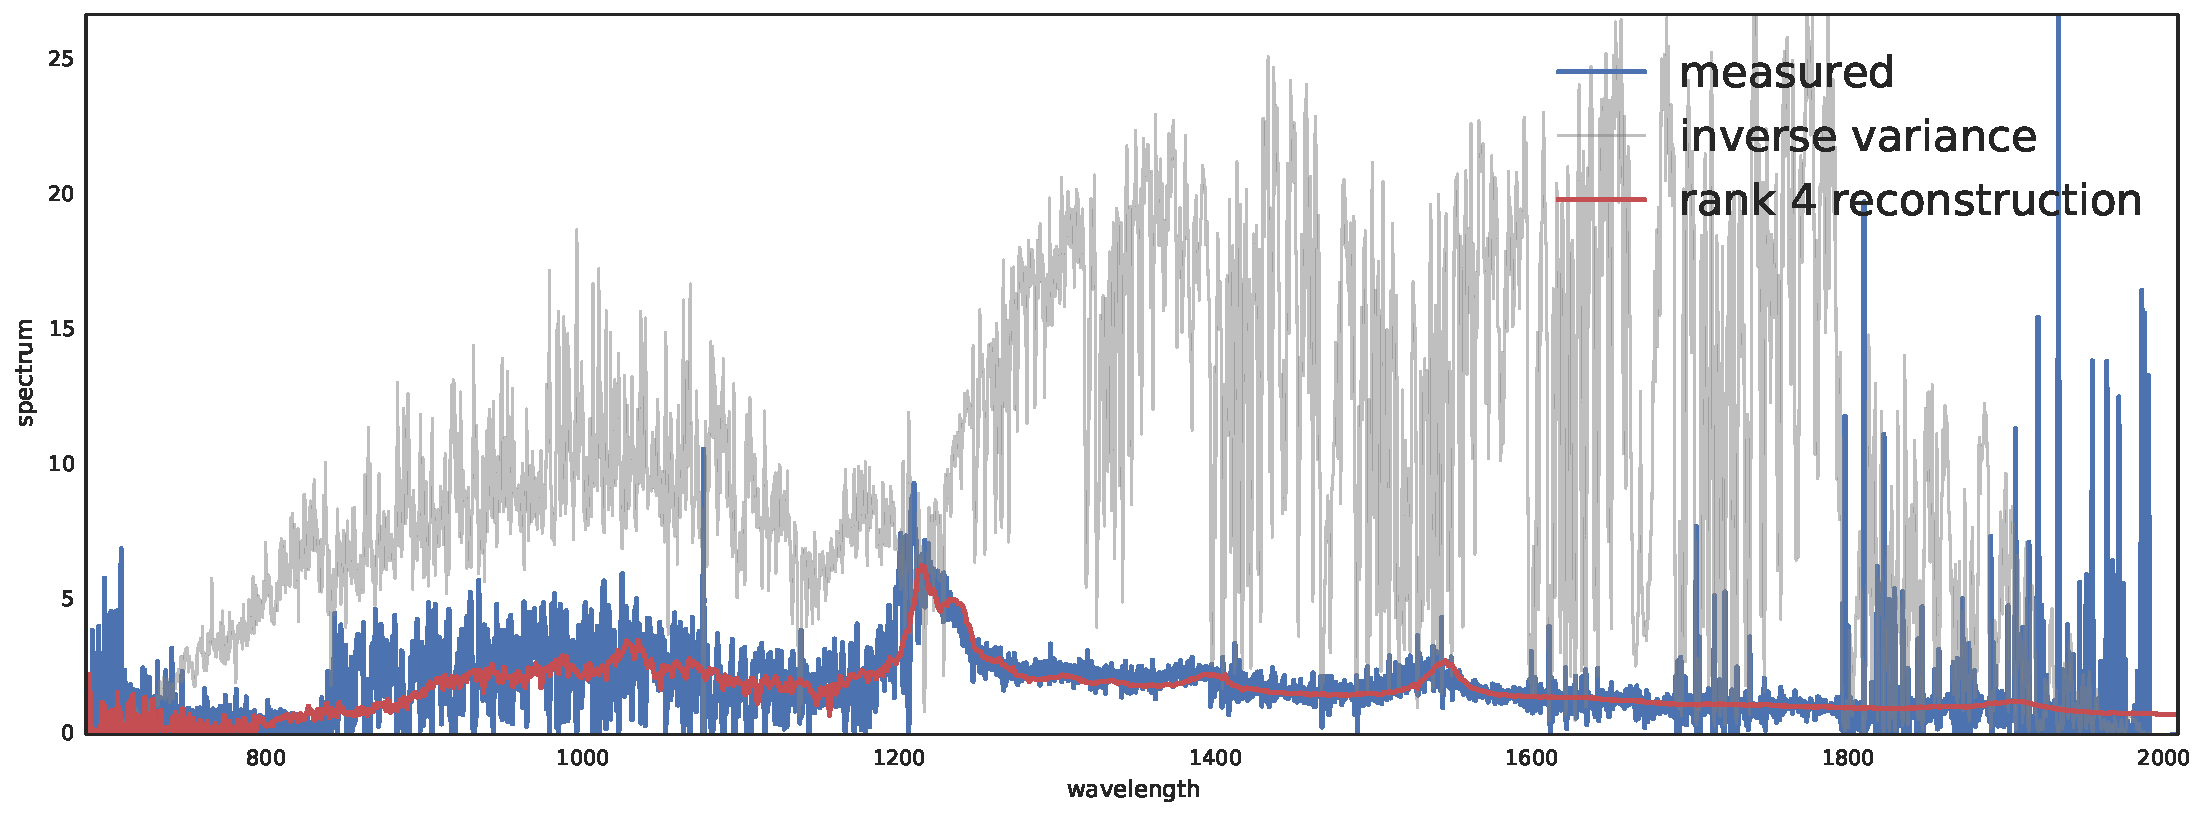
\includegraphics[width=.99\textwidth]{../figs/idx_4_rank_4_reconstruction.pdf}
\vskip -.2in
\end{figure}


%---------------

\paragraph{SED Basis}
We depict a MAP estimate of $B_1, \dots, B_k$ in Figure~\ref{fig:basis}.
Our basis decomposition enjoys the benefit of physical interpretability due to our density-estimate formulation of the problem.
Bases $B_1, B_2$ place mass on the Lyman-$\alpha$ peak around 1,216~$\angstrom$, allowing the model to capture the co-occurrence of more peaked SEDs with a bump around 1,550~$\angstrom$.  
Furthermore, because of the flexible nonparametric priors on $B_k$ our model automatically learned this feature from the data.
The positivity of the basis and weights distinguishes our model from PCA-based methods, which sacrifice physical interpretability.   

\paragraph{Photometric measurements}
For each test quasar, we construct an 8-chain parallel tempering sampler and run for 8,000 iterations, and discard the first 4,000 samples as burn-in. 
%Given posterior samples of~$z_n$, we formulate two point estimates: the posterior mean and the location with highest posterior mode.
%To determine this location, we choose the sample with highest probability under a kernel density estimate of the samples with a fixed bandwidth, ${\beta = .08}$.  
Given posterior samples of~$z_n$, we take the posterior mean as a point estimate.  
Figure~\ref{fig:vs} compares the posterior mean to spectroscopic measurements (for three different data-split experiments), where the gray lines denote posterior sample quantiles. 

We see that in general there is a strong correspondence between spectroscopically measured redshift and our posterior estimate.
In cases where the posterior mean is off, our distribution often covers the spectroscopically confirmed value with probability mass.
This is clear upon inspection of posterior marginal distributions that exhibit extreme multi-modal behavior.  
To combat this multi-modality, it is necessary to inject the model with more information to eliminate plausible hypotheses; this information could come from another measurement (e.g., a new photometric band), or from structured prior knowledge over the relationship between $z_n, \mathbf{w}_n$, and $m_n$.  Our method simply fits independent mixtures of Gaussians to spectroscopically confirmed data to formulate a prior distribution.  However, incorporating dependencies between $z_n$, $\mathbf{w}_n$ and $m_n$, similarly to the XDQSOz technique, will be incorporated in future work. 



%----- Red Shift, spec vs photo -------------------------------------------------
\begin{figure}[t]
\vskip -.16in
\begin{center}
  \includegraphics[height=.34\textwidth]{{scatter_exp-random}.pdf}
  \includegraphics[height=.34\textwidth]{{scatter_exp-flux}.pdf}
  \includegraphics[height=.34\textwidth]{{scatter_exp-redshift}.pdf}
\end{center}
\vskip -.16in
\caption{%
Comparison of spectroscopically ($x$-axis) and photometrically ($y$-axis) measured redshifts from the SED model for three different data splits.  The left reflects a random selection of 4,000 quasars from the DR10QSO dataset.  The right graph reflects a selection tof 4,000 test quasars from the upper 15\% ($z_{cutoff} \approx 2.7$), where all training was done on lower redshifts.  The red estimates are posterior means. 
}
\label{fig:vs}
\end{figure}
%-------------------------------------------------------
%-----  -------------------------------------------------
\begin{figure*}[t]
\vskip -.16in
\centerline{
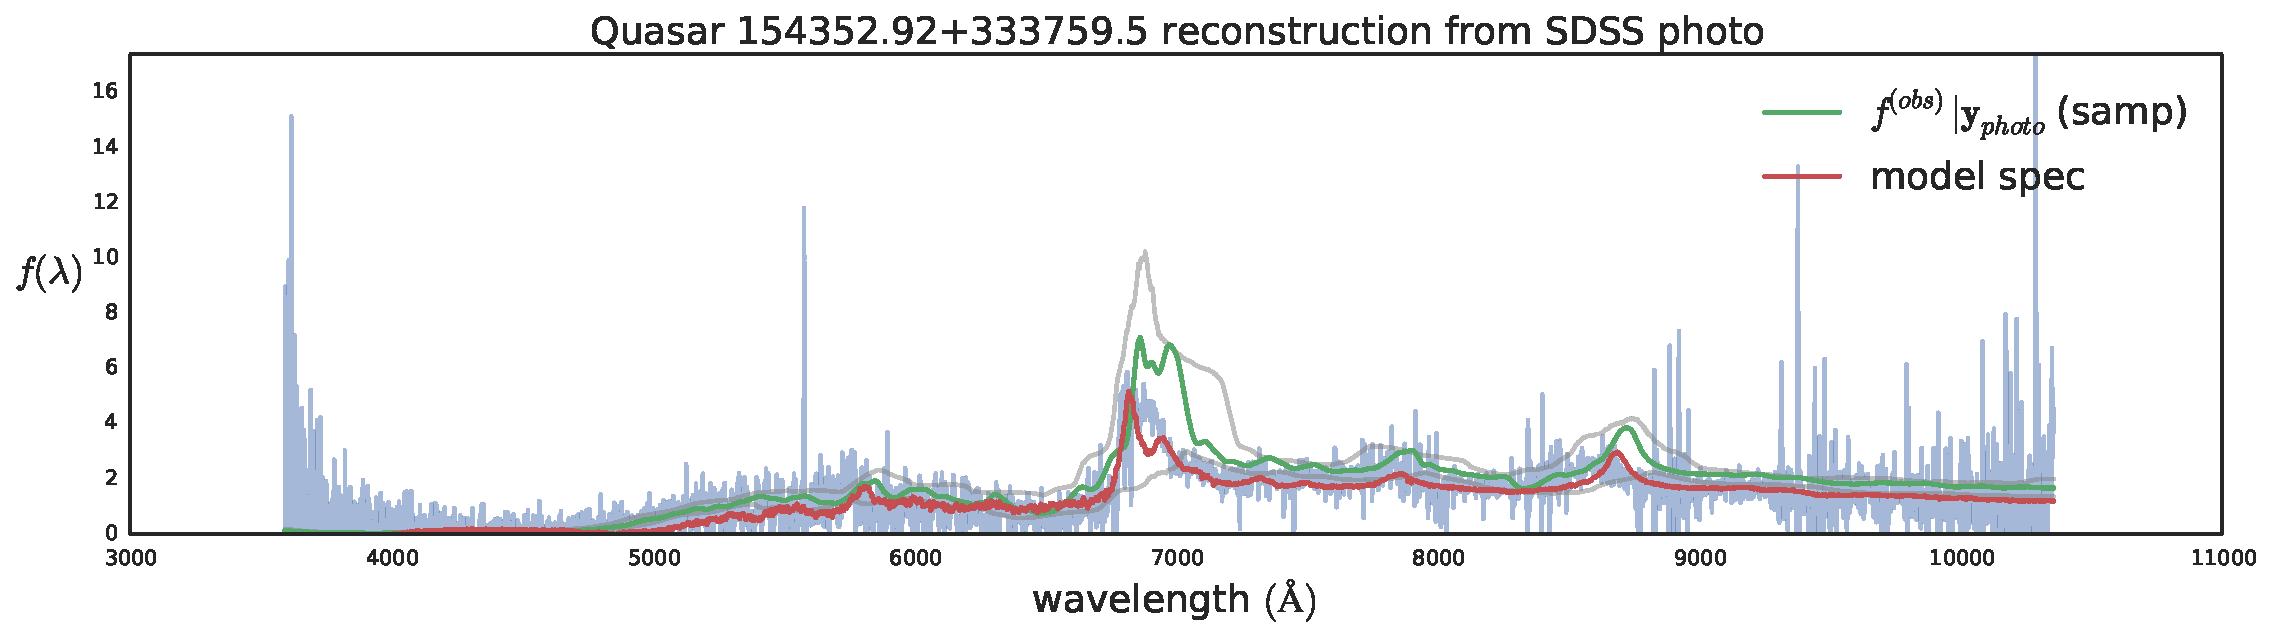
\includegraphics[height=.22\textwidth]{../figs/quasar_plots/quasar_490_mcmc_recon.pdf}
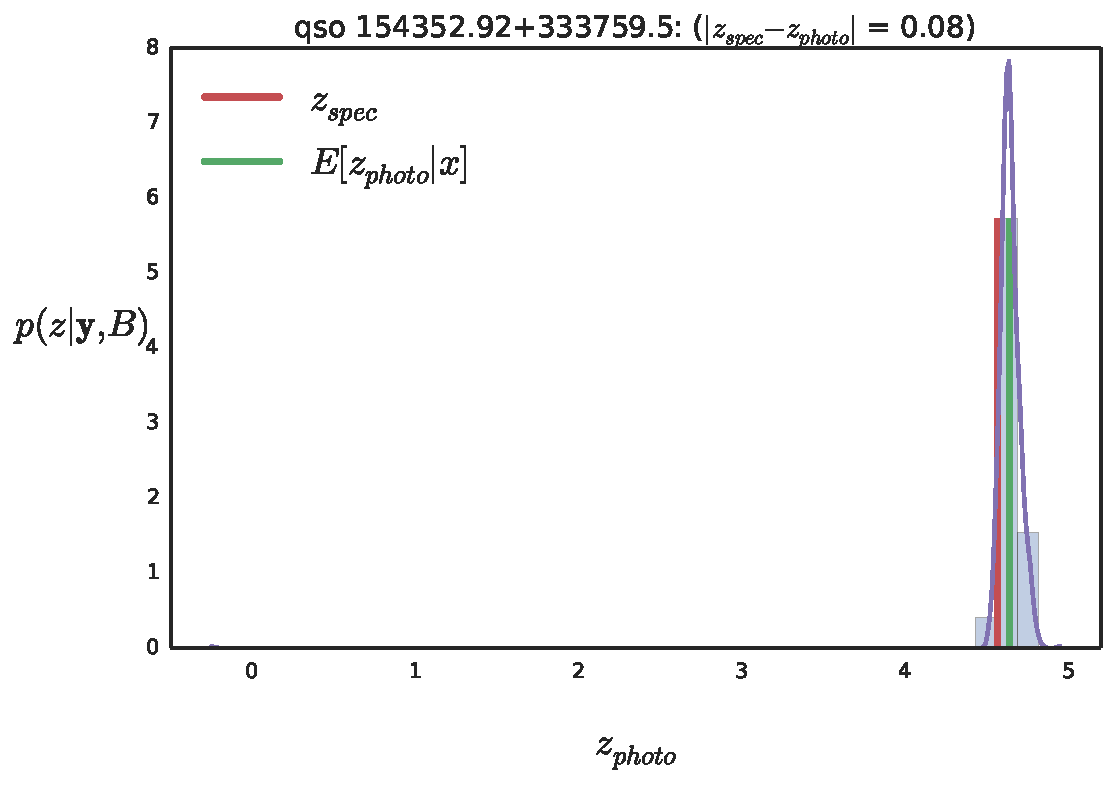
\includegraphics[height=.22\textwidth]{../figs/quasar_plots/quasar_490_posterior_z}
} 
\centerline{
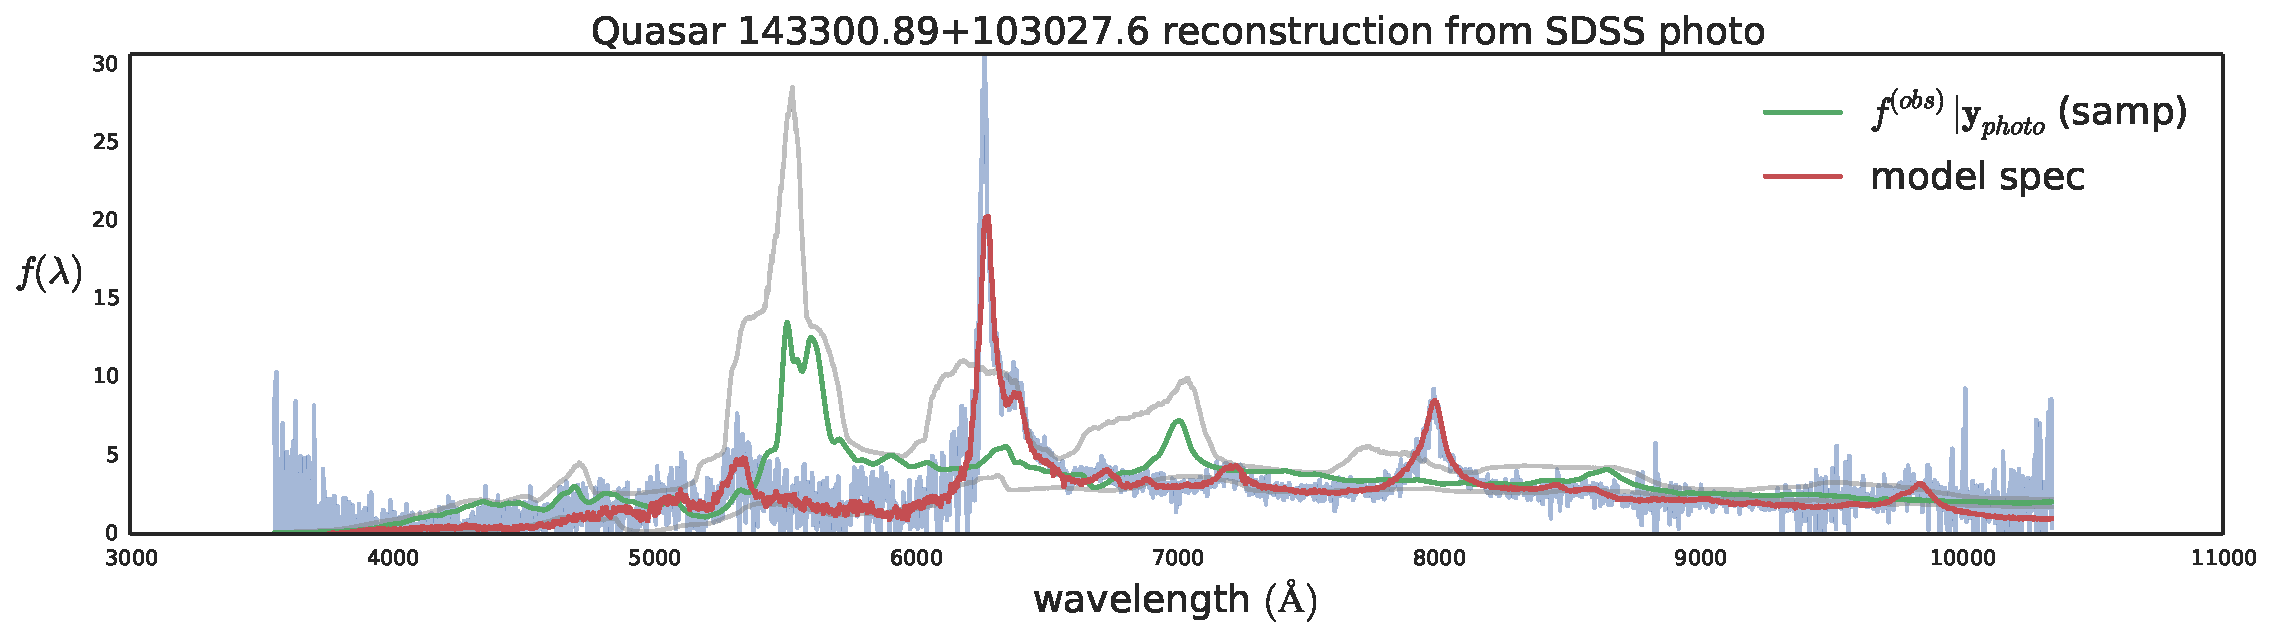
\includegraphics[height=.22\textwidth]{../figs/quasar_plots/quasar_214_mcmc_recon.pdf}
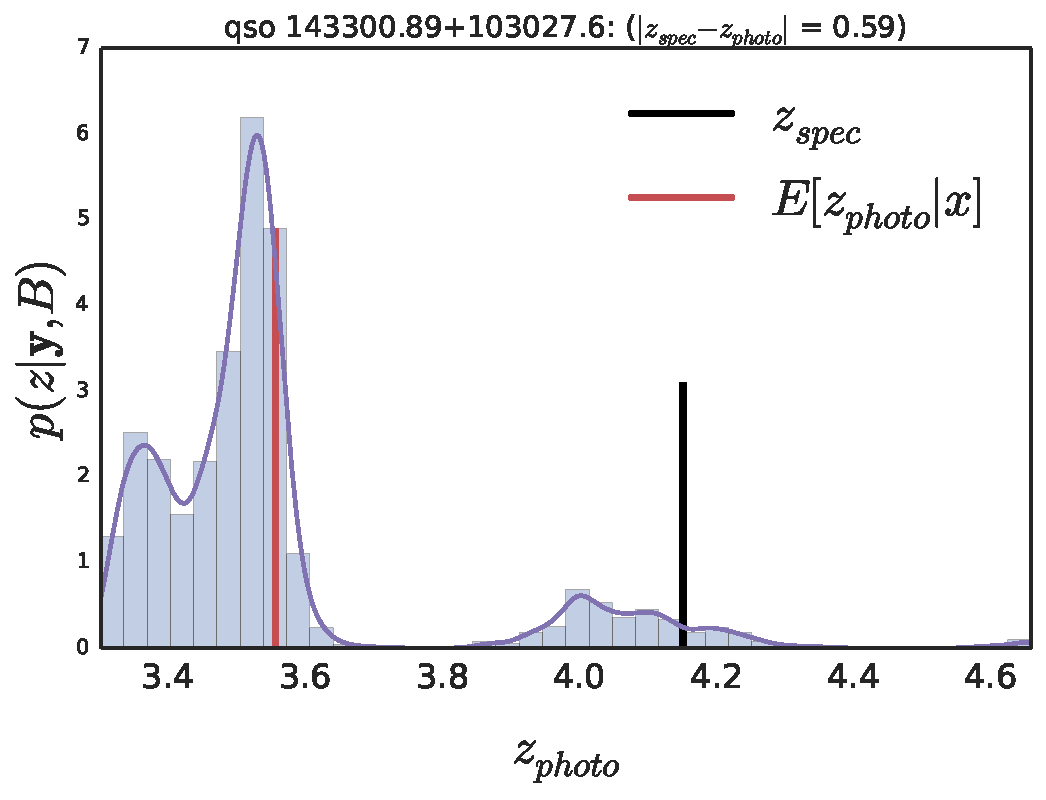
\includegraphics[height=.22\textwidth]{../figs/quasar_plots/quasar_214_posterior_z}
}
\caption{Left: inferred SEDs from photometric data.  
The black line is a PCA-based model fit to the full spectral data.  
The red line is a sample from the posterior, $f^{(obs)}_n(\lambda) | \mathbf{X}, \mathbf{y}_n, B$, which imputes the entire SED from only five flux measurements.  
Note that the bottom sample is from the left mode, which under-predicts redshift.   
Right: corresponding posterior predictive distributions, $p(z_n | \mathbf{X}, \mathbf{y}_n, B)$.  The black line marks the spectroscopically confirmed redshift; the red line marks the posterior mean. Note the difference in scale of the $x$-axis.}
\label{fig:recon}
\vskip -0.1in
\end{figure*}
%---------------

\subsection{Comparisons}
We compare the performance of our redshift estimator with two recent photometric redshift estimators, XDQSOz \cite{bovy2012photometric} and a neural network \cite{brescia2013photometric}.
The method in \cite{bovy2012photometric} is a conditional density estimator that discretizes the range of one flux band (the $i$-band) and fits a mixture of Gaussians to the joint distribution over the remaining fluxes and redshifts. 
One disadvantage to this approach is there there is no physical significance to the mixture of Gaussians. 
Furthermore, the original method trains and tests the model on a pre-specified range of $i$-magnitudes, which is problematic when predicting redshifts on much brighter or dimmer stars. 
The method from \cite{brescia2013photometric} employs a neural network with two hidden layers, and the SDSS fluxes as inputs
More features (e.g., more photometric bands) can be incorporated into all models, but we limit our experiments to the five SDSS bands for the sake of comparison.  
Further detail on these two methods and a broader review of ``photo-z'' approaches are available in the supplementary material.  

\paragraph{Average error and test distribution}
We compute mean absolute error (MAE), mean absolute percentage error (MAPE), and root mean square error (RMSE) to measure predictive performance.  
Table~\ref{tab:error} compares prediction errors for the three different approaches (XD, NN, Spec). %We also quantify average prediction error and posterior quantile interval coverage for sets of quasars with increasing redshift.  
Our experiments show that accurate redshift measurements are attainable even when the distribution of training set is different from test set by directly modeling the SED itself. Our method dramatically outperforms \cite{bovy2012photometric} and \cite{brescia2013photometric} in split (iii), particularly for very high redshift fluxes.  
We also note that our training set is derived from only 2,000 examples, whereas the training set for XDQSOz and the neural network were $\approx$ 80,000 quasars and 50,000 quasars, respectively.  This shortcoming can be overcome with more sophisticated inference techniques for the non-negative basis.  Despite this, the SED-based predictions are comparable.
  
Furthermore, because we are directly modeling the latent SED, our method admits a posterior estimate of the entire SED.
Figure~\ref{fig:recon} displays posterior SED samples and their corresponding redshift marginals for test-set quasars inferred from only SDSS photometric measurements.  
Our experiments suggest that the SED-based model using a physical generative process will make better predictions for quasars with very different properties from the training set.

%---- TABLE --------------------------------------
\begin{table*}[t]
\caption{Prediction error for three train-test splits, (i) random, (ii) flux-based, (iii) redshift-based, corresponding to XDQSOz \cite{bovy2012photometric} (XD), the neural network approach \cite{brescia2013photometric} (NN), our SED-based model (Spec). The middle and lowest sections correspond to test redshifts in the upper 50\% and 10\%, respectively.  The XDQSOz and NN models were trained on (roughly) 80,000 and 50,000 example quasars, respectively, while the Spec models were trained on 2,000. }
\label{tab:error}
\begin{center}
\begin{small}

\begin{tabular}{ p{2.9cm}|ccc|ccc|ccc}
 & \multicolumn{3}{c}{MAE} & \multicolumn{3}{c}{MAPE} & \multicolumn{3}{c}{RMSE} \\
 \hline
 split & XD & NN & Spec & XD & NN & Spec & XD & NN & Spec \\
 \hline
 random (all) & \textbf{0.359} & 0.773 & 0.485 & \textbf{0.293} & 0.533 & 0.430 & \textbf{0.519} & 0.974 & 0.808  \\
 flux (all) & \textbf{0.308} & 0.483 & 0.497 & \textbf{0.188} & 0.283 & 0.339 & \textbf{0.461} & 0.660 & 0.886  \\
 redshift (all) & 0.841 & 0.736 & \textbf{0.619} & 0.237 & 0.214 & \textbf{0.183} & 1.189 & 0.923 & \textbf{0.831}  \\
 \hline
 random ($z > 2.35$) & \textbf{0.247} & 0.530 & 0.255 & \textbf{0.091} & 0.183 & 0.092 & \textbf{0.347} & 0.673 & 0.421  \\
 flux ($z > 2.33$) & \textbf{0.292} & 0.399 & 0.326 & \textbf{0.108} & 0.143 & 0.124 & \textbf{0.421} & 0.550 & 0.531  \\
 redshift ($z > 3.20$) & 1.327 & 1.149 & \textbf{0.806} & 0.357 & 0.317 & \textbf{0.226} & 1.623 & 1.306 & \textbf{0.997}  \\
 \hline
 random ($z > 3.11$) & \textbf{0.171} & 0.418 & 0.289 & \textbf{0.050} & 0.117 & 0.082 & \textbf{0.278} & 0.540 & 0.529  \\
 flux ($z > 2.86$) & 0.373 & 0.493 & \textbf{0.334} & 0.112 & 0.144 & \textbf{0.103} & \textbf{0.606} & 0.693 & 0.643  \\
 redshift ($z > 3.80$) & 2.389 & 2.348 & \textbf{0.829} & 0.582 & 0.569 & \textbf{0.198} & 2.504 & 2.405 & \textbf{1.108}  \\
 \hline
\end{tabular}

\end{small}
\end{center}
\vskip -.16in
\end{table*}
\vskip -.16in

%----------------------------------------------------------------------------------
%----------------------------------------------------------------------------------
%----------------------------------------------------------------------------------
\section{Discussion}
We have presented a generative model to combine two sources of information at very different spectral resolutions to form an estimate of the latent spectral energy distribution of quasars.
We described the details of the model, its implied structure, and a computationally tractable MCMC-based inference algorithm. 
Our model accurately predicts and characterizes uncertainty about redshifts from only photometric observations and a small number of separate spectroscopic examples. 
%Our experiments showed the utility of our model for the task of inferring quasar redshift from photometric data, showing that we can accurately predict and characterize uncertainty about redshift values with a small number of spectroscopic examples.  
Moreover, we showed that we can make reasonable estimates of the unobserved SED itself, from which we can make inferences about other physical properties informed by the full SED.  
 
We see multiple avenues of future work.
Firstly, we can extend the model of SEDs to incorporate more expert knowledge.
One such augmentation would include a fixed collection of features, curated by an expert, corresponding to physical properties already known about a class of sources.  
We can also extend our model to directly incorporate photometric pixel observations.
Our current specification uses the output of a photometric preprocessing step, however, a logical extension is to model photon counts at the pixel level and perform inference over a joint model. 
Because pixel appearance models conditioned on the SED of a source are well-known, we see this as a feasible next step. 

%We can also extend our model to include information from different sources of photometry and spectroscopy.
%Other photometric surveys measure different ranges of the spectrum, yielding more information about the underlying SED.
%Methods that incorporate photometry from different sources have been shown to improve redshift estimates \cite{brescia2013photometric}.  
Secondly, we note that our method is more more computationally burdensome than XDQSOz and the neural network approach.  Another avenue of future work is to find accurate approximations of these posterior distributions that are cheaper to compute. 

Lastly, we can extend our methodology to galaxies, whose SEDs can be quite complicated.
For instance, galaxy observations have spatial extent and they are therefore not well modeled as a single point in the sky.  
Models for spatial extent have been developed and applied to photometric data \cite{hogg2013replacing, regier2015}.  
However, a galaxy's SED can vary spatially, presenting a more complex modeling task.    
The combination of SED and spatial appearance modeling and computationally efficient inference procedures is a promising route toward the automatic characterization of millions of sources from the enormous amounts of data available in massive photometric surveys.  

% Acknowledgements should only appear in the accepted version. 
%\textbf{Do not} include acknowledgements in the initial version of
%the paper submitted for blind review.
%\section*{Acknowledgments} 
%This work is supported by the Applied Mathematics Program within the Office of Science Advanced Scientific Computing Research of the U.S. Department of Energy under contract No. DE-AC02-05CH11231. This work used resources of the National Energy Research Scientific Computing Center (NERSC). We would like to thank Tina Butler, Tina Declerck and Yushu Yao for their assistance.

% ACM: thank dougal and scott for code
%If a paper is accepted, the final camera-ready version can (and
%probably should) include acknowledgements. In this case, please
%place such acknowledgements in an unnumbered section at the
%end of the paper. Typically, this will include thanks to reviewers
%who gave useful comments, to colleagues who contributed to the ideas, 
%and to funding agencies and corporate sponsors that provided financial 
%support.  

% In the unusual situation where you want a paper to appear in the
% references without citing it in the main text, use \nocite
%\nocite{langley00}


\bibliographystyle{plain}
\bibliography{../refs}
\end{document}
